\ofsubsection{Triple Triad}
%
\ofquote{"I knew we were destined to play. Let's begin!"\\}{Quistis}
%
\begin{center} 
\includegraphics[width=\columnwidth]{./art/tripletriad/board.jpg} \end{center}
%
\accf{Triple Triad} is a card game that was invented by the psychic Orlan, inspired by tarot cards.
At first, it was played by soldiers to pass time, but eventually became popular with people of all ages and occupations.
Before staring a game of Triple Triad, each player chooses a hand of 5 cards from his collection.
The GM decides who goes first and both players take alternating turns until the game ends.
During each turn, a player has to place one card on an empty space on a 3-by-3 board. 
Every Triple Triad card has a number on each of its four sides and when you place a card next to one of your opponent's, the numbers on the touching sides are compared.
If your number is higher, you capture the other card.
Players can only capture cards during their turn, a card that was just placed cannot be captured.
You can place small tokens to keep track of who currently owns which cards on the board.
The goal is to capture as many cards as possible and after the board is completely filled, the player with the most cards in his possession wins the game.
Cards that are still in your hand also contribute to your total score.
When the final score is tied, the game is started from the beginning, until one player wins.
While the rules above always apply, additional rules may be used by some players depending on the location.
Below are some of the most common special rules.
%
\vfill
%
\oftable{p{0.15\columnwidth} p{0.8\columnwidth}}
{\accf{Rule} & \accf{Description}} {
	Open &  Both players play with open hands.\ofrow
	Same & When you place a card next to one with the same number on the touching side, you still capture it.\ofrow
	Combo & When you capture a card, then you also capture all of its other adjacent cards that have a lower number than it does on the respective touching sides. The rule is then applied to all further captured cards.\ofrow
	Random & Players cannot choose their hand. Instead they draw 5 random cards from their collection. \ofrow
	Sudden \newline Death & In case of a draw, the game is restarted and both players use their captured cards from the previous game as their hand.
}
%
\newpage
%
\ofquote{"I can tell you have collected and played cards all over the world. And you remind me of her... Her talent especially. Oh, now I have said too much."\\}{Prince Spade}\\\\
%
While Triple Triad tournaments usually award Gil, Items or Equipment for winning, casual games focus on acquiring new cards.
With the most commonly used rule, the winner takes one card of his or her choice from the loser's hand.
However, there are also different rules for card rewards, some of which are listed below.
In addition, cards may also be bought, sold and traded just as any other good.
Prices may vary significantly depending on the popularity of the game and the rarity of the card.
%
\\\\
%
\oftable{p{0.15\columnwidth} p{0.8\columnwidth}}
{\accf{Rule} & \accf{Description}} {
    Diff & Winner takes an amount of cards from the opponent's hand equal to the difference of their final scores.\ofrow	
    Direct & Both players take all cards that are in their possession at the end of the game. \ofrow	
	All & Winner takes all 5 cards from the loser's hand.
}
%
\vfill
%
%	
\begin{center} 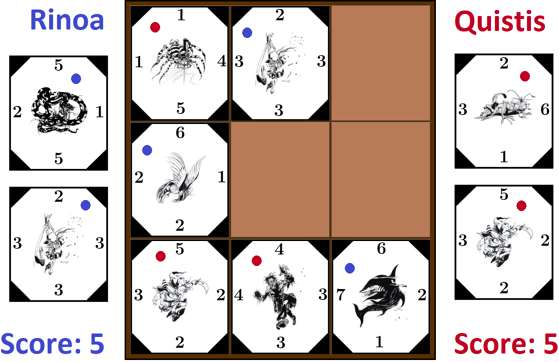
\includegraphics[width=1\columnwidth]{./art/tripletriad/example.jpg} \end{center}
%
In the example above, both players have already placed 3 cards and the score is tied.
The colored markers on the cards indicate which player currently owns which cards.
It is Quistis' turn, so she has to play one of the two cards in her hand onto one of the free spaces.
A strong move would be to place the Goblin card (the bottom one) in the central space, as that would allow Quistis to capture both the center-top and the center-left cards.
Another smart move would be to place the basilisk card (the top one) in the central space, which would only capture the center-left card, but have a stronger defense against the open space on the center-right.
Quistis could also safely place any of the two cards in one of the other two free spaces, but in this situation it would not allow her to capture any of Rinoa's cards. 
Below is a list of Triple Triad cards that is sorted by card rarity from top to bottom.
%At its end, there is a page with backsides, which you can use to print both sides of the cards.
%
\clearpage
%
\newgeometry{bottom=2mm,top=2mm,right=5mm,left=5mm}	
\setlength{\columnsep}{11cm}

\newcommand{\cardback}[0]
{
	
\includegraphics[width=6cm]{./art/tripletriad/cardback.jpg}
	\vskip0.445cm
}

\newcommand{\card}[1]
{
	\includegraphics[width=6cm]{./art/tripletriad/#1.jpg}
	\vskip0.4cm
}
%
\begin{multicols}{3}[][20cm]
%
%col1
\card{l1_astos}
\card{l1_parasite}
\card{l2_helldiver}
\card{l2_worm}
%col2
\card{l1_cobra}
\card{l1_spider}
\card{l2_sahagin}
\card{l3_cockatrice}
%col3
\card{l1_goblin}
\card{l2_bloodsucker}
\card{l2_skeleton}
\card{l3_mantis}
%
\clearpage
%
%col1
\card{l3_nitemare}
\card{l4_eye}
\card{l4_pirate}
\card{l5_ankylo}
%col2
\card{l3_zombie}
\card{l4_gargoyle}
\card{l4_soldier}
\card{l5_deadringer}
%col3
\card{l4_cerberus}
\card{l4_ghost}
\card{l5_adamantoise}
\card{l5_gigas}
%
\clearpage
%
%col1
\card{l5_shark}
\card{l6_medusa}
\card{l7_behemoth}
\card{l7_ochu}
%col2
\card{l6_chimera}
\card{l6_troll}
\card{l7_bull}
\card{l7_witch}
%col3
\card{l6_manticore}
\card{l6_wizard}
\card{l7_giant}
\card{l8_deadrider}
%
\clearpage
%
%col1
\card{l8_ghost}
\card{l9_badman}
\card{l9_vampire}
\card{l10_lich}
%col2
\card{l8_hydra}
\card{l9_dragon}
\card{l10_kraken}
\card{l10_tiamat}
%col3
\card{l8_mancat}
\card{l9_malboro}
\card{l10_marilith}
\card{l10_chaos}
%
\clearpage
%
%\cardback
%\cardback
%\cardback
%\cardback
%\cardback
%\cardback
%\cardback
%\cardback
%\cardback
%\cardback
%\cardback
%\cardback

\end{multicols}

\restoregeometry
\pagebreak